%----------------------------------------------------------------------------------------
%    PACKAGES AND THEMES
%----------------------------------------------------------------------------------------

\documentclass[aspectratio=169,xcolor=dvipsnames]{beamer}
\usetheme{SimpleDarkBlue}

\usepackage{hyperref}
\usepackage{graphicx} % Allows including images
\usepackage{booktabs} % Allows the use of \toprule, \midrule and \bottomrule in tables

\usepackage{caption} % Allows the usage of \captionsetup
\DeclareCaptionFormat{nolabel}{#3} % Removes "Listing:" prefix
\captionsetup[lstlisting]{format=nolabel}

\usepackage{enumitem}
\setlist[itemize,1]{label=\textbullet}
\setlist[itemize,2]{label=--}

\usepackage[T1]{fontenc}
\usepackage{cascadia-code}

\usepackage{xcolor}
\definecolor{codegreen}{rgb}{0,0.6,0}
\definecolor{codegray}{rgb}{0.5,0.5,0.5}
\definecolor{codepurple}{rgb}{0.58,0,0.82}
\definecolor{backcolour}{rgb}{0.9,0.9,0.9}

\usepackage{listings}
\lstdefinestyle{mystyle}{
    backgroundcolor=\color{backcolour},
    commentstyle=\color{codegreen},
    keywordstyle=\color{magenta},
    numberstyle=\tiny\color{codegray},
    stringstyle=\color{codepurple},
    basicstyle=\ttfamily\footnotesize,
    breakatwhitespace=false,
    breaklines=true,
    captionpos=b,
    keepspaces=true,
    numbers=left,
    numbersep=5pt,
    showspaces=true,
    showstringspaces=true,
    showtabs=true,
    tabsize=4,
    aboveskip=0pt, % Reduce space above
    belowskip=0pt  % Reduce space below
}
\lstset{style=mystyle}

%----------------------------------------------------------------------------------------
%    TITLE PAGE
%----------------------------------------------------------------------------------------

\title{Ateliers Créactifs Raspberry Pi}
\subtitle{Explication des HATs et création d'une borne d'arcade.}

\author{Jean Bourgies, François Marelli, Ugo Proietti}

\date{10 mars 2025}

%----------------------------------------------------------------------------------------
%    PRESENTATION SLIDES
%----------------------------------------------------------------------------------------

\begin{document}

\begin{frame}
    % Print the title page as the first slide
    \titlepage
\end{frame}

\begin{frame}{Table des matières}
    % Throughout your presentation, if you choose to use \section{} and \subsection{} commands, these will automatically be printed on this slide as an overview of your presentation
    \tableofcontents
\end{frame}

%------------------------------------------------
\section{Explication des HATs}
%------------------------------------------------

\begin{frame}{HATs ?}
    \begin{columns}[c] % 'c' ensures vertical centering for both columns

        \column{1\textwidth}
        \begin{itemize}
            \item Hardware Attached on Top / matériel attaché sur le dessus.
            \item Extensions prévues pour les RPI (connectique et dimensions).
            \item Permet d'étendre les fonctionalités de base du RPI.
        \end{itemize}

    \end{columns}
\end{frame}

\begin{frame}
    \begin{columns}[c] % 'c' ensures vertical centering for both columns

        \column{0.5\textwidth}
        \begin{figure}
            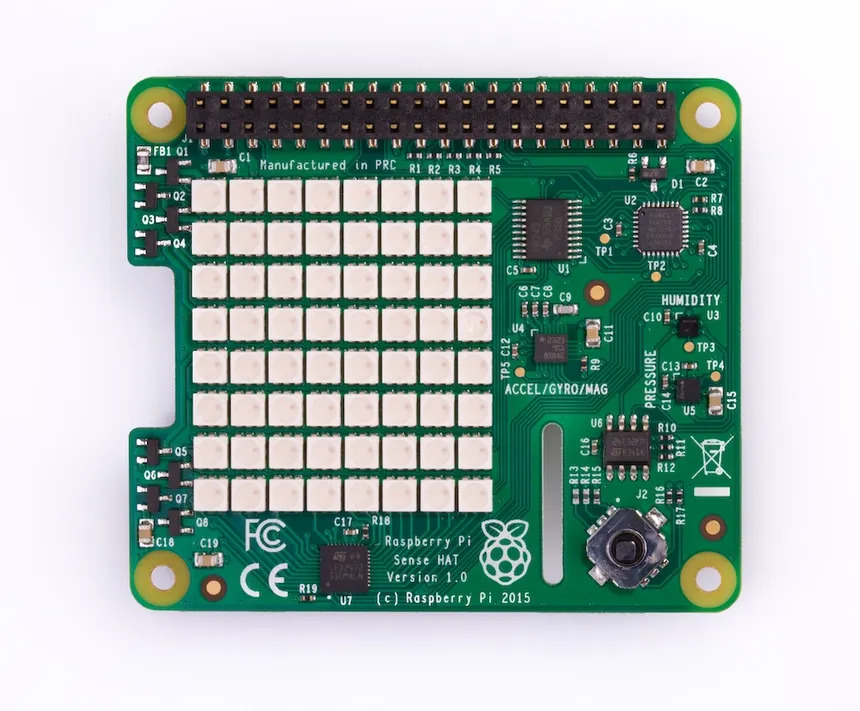
\includegraphics[width=0.5\textwidth]{images/sense_hat.jpg}
            \captionsetup{labelformat=empty}
            \caption{Sense HAT}

            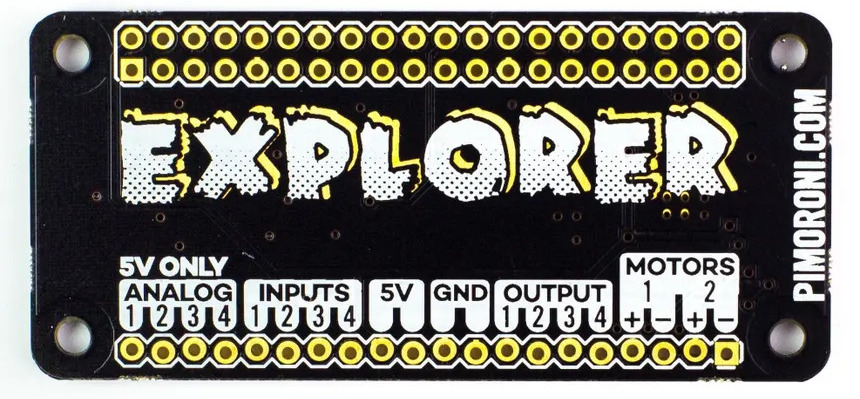
\includegraphics[width=0.5\textwidth]{images/explorer_hat.jpg}
            \captionsetup{labelformat=empty}
            \caption{Explorer HAT}
        \end{figure}

        \column{0.5\textwidth}
        \begin{figure}
            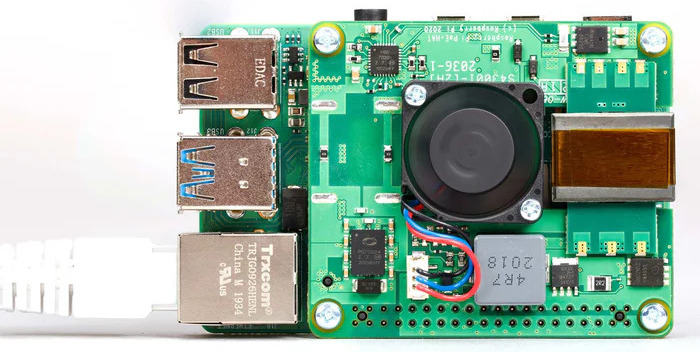
\includegraphics[width=0.5\textwidth]{images/poe_hat.jpg}
            \captionsetup{labelformat=empty}
            \caption{PoE HAT}

            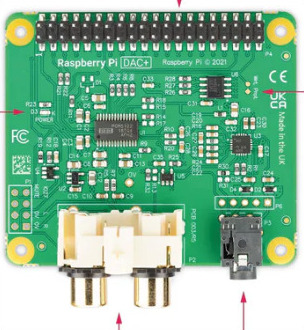
\includegraphics[width=0.5\textwidth]{images/dac_hat.jpg}
            \captionsetup{labelformat=empty}
            \caption{DAC+ HAT}
        \end{figure}

    \end{columns}
\end{frame}

\begin{frame}{HAT pour une borne d'arcade}
    \begin{columns}[c] % 'c' ensures vertical centering for both columns

        \column{.5\textwidth} % Left column
        \begin{figure}
            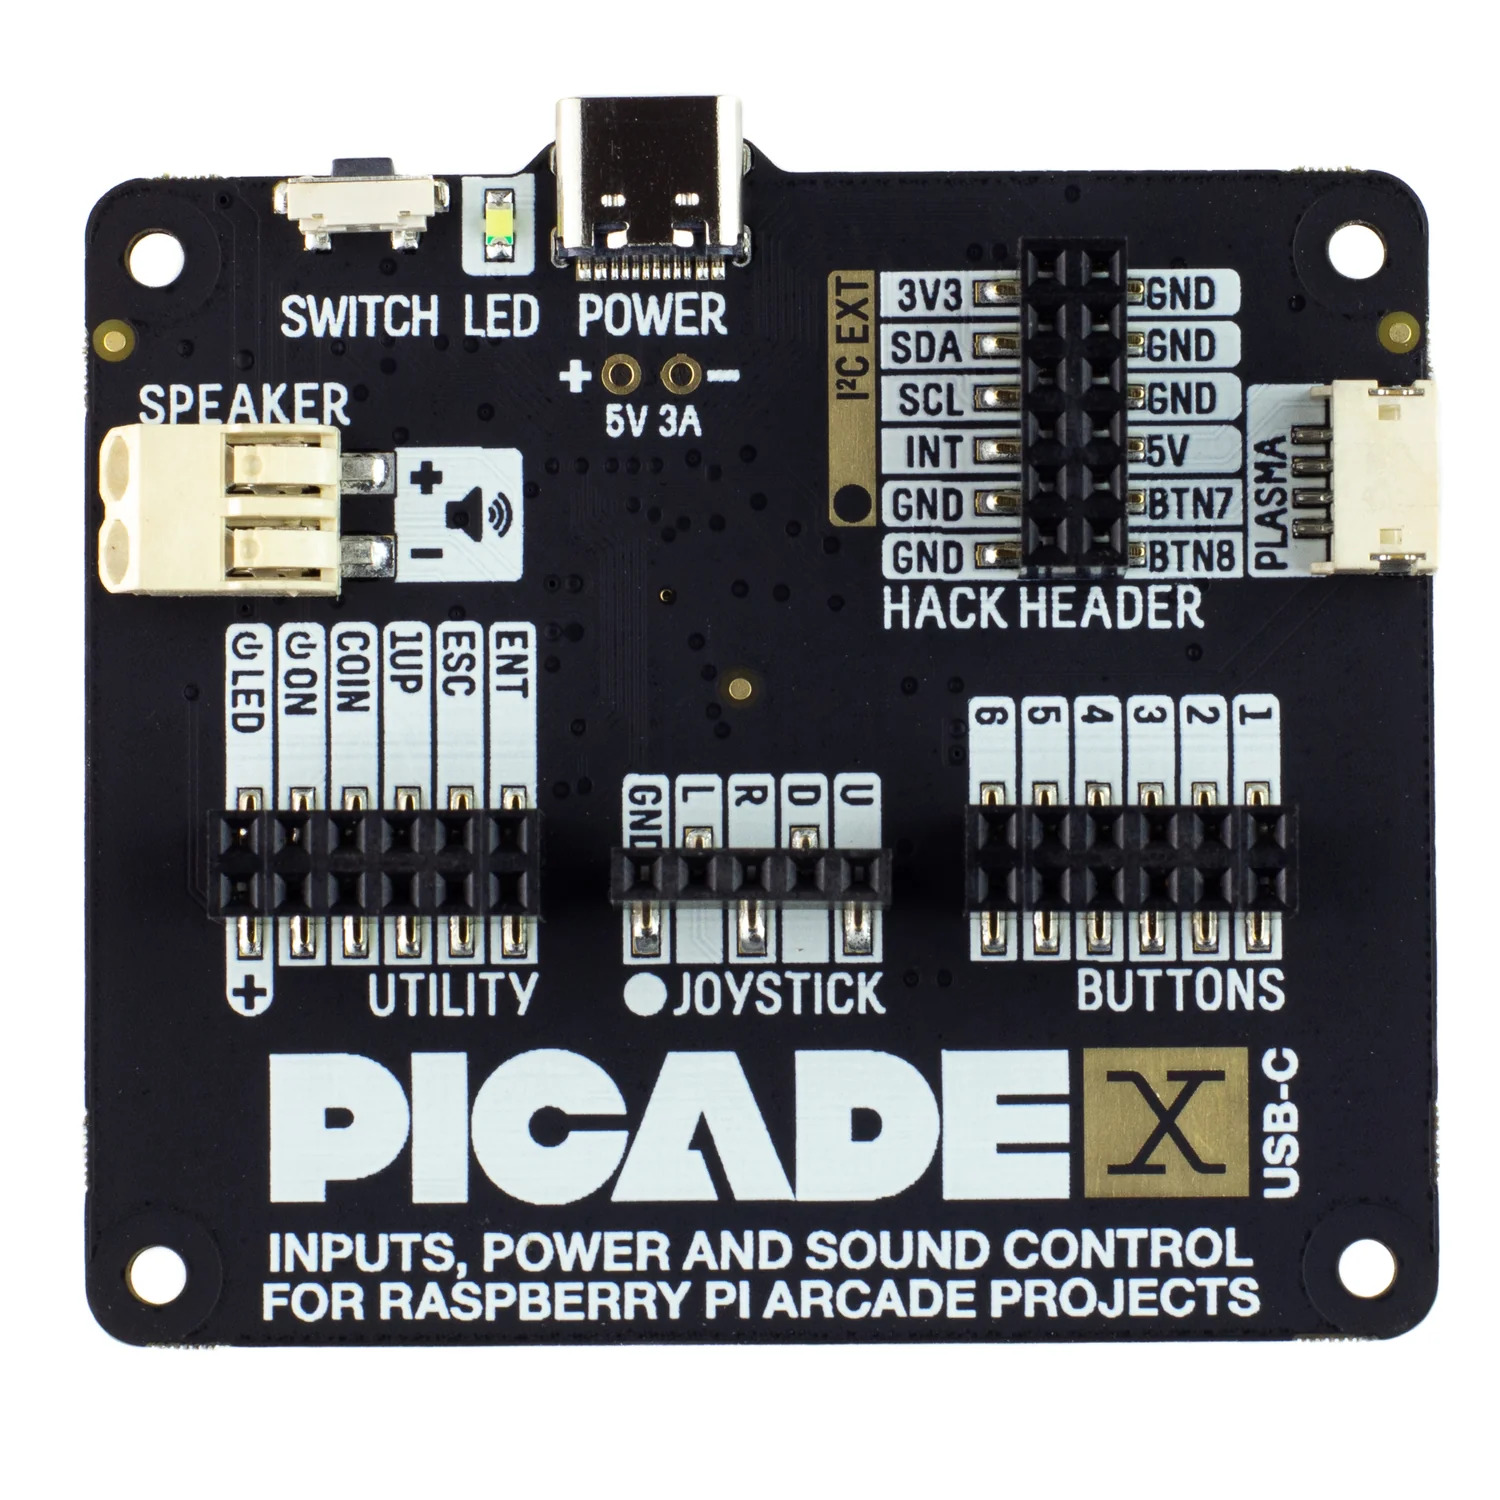
\includegraphics[width=0.8\textwidth]{images/picade_hat.jpg}
        \end{figure}

        \column{.5\textwidth} % Right column
        \begin{itemize}
            \item Picade X.
            \item Solution tout en un pour les bornes d'arcade.
            \item Gestion des joystick, boutons, haut-parleur, alimentation.
        \end{itemize}

    \end{columns}
\end{frame}

\begin{frame}{Port PCIe}
    \begin{columns}[c] % 'c' ensures vertical centering for both columns

        \column{.6\textwidth} % Left column
        \begin{figure}
            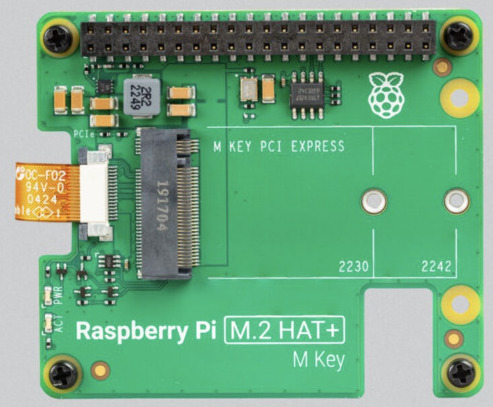
\includegraphics[width=1\textwidth]{images/pcie_hat_top.jpg}
        \end{figure}

        \column{.4\textwidth} % Right column
        \begin{itemize}
            \item À partir du RPI5.
            \item Port PCIe.
            \item Grandes performances.
            \item Compatible avec beaucoup de matériel informatique.
        \end{itemize}

    \end{columns}
\end{frame}

\begin{frame}
    \begin{columns}[c] % 'c' ensures vertical centering for both columns

        \column{0.5\textwidth}
        \begin{figure}
            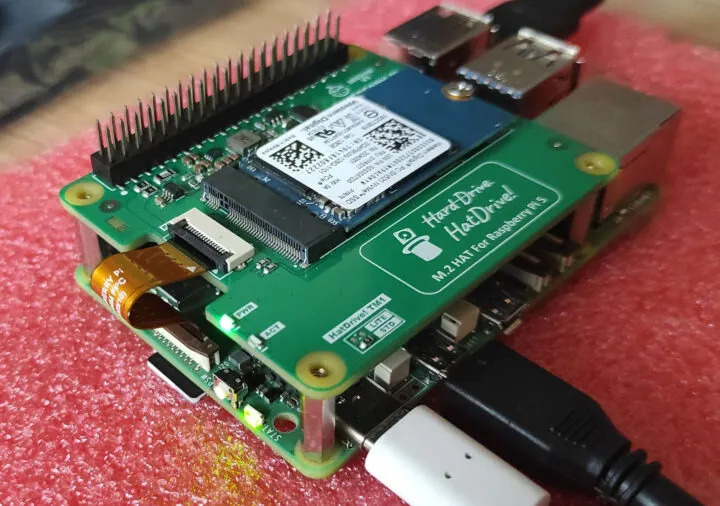
\includegraphics[width=0.7\textwidth]{images/pcie_hat.jpg}
        \end{figure}
        \begin{figure}
            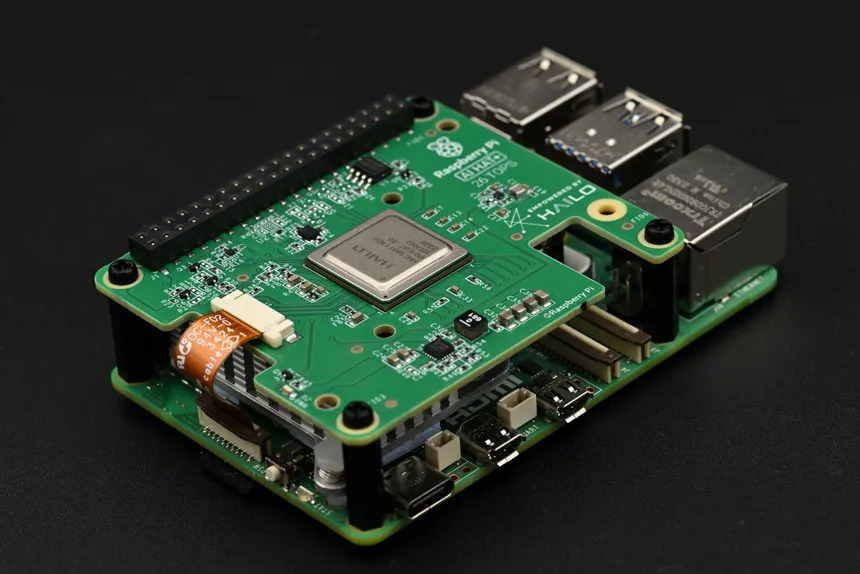
\includegraphics[width=0.7\textwidth]{images/pcie_ai_hat.jpg}
        \end{figure}

        \column{0.5\textwidth}
        \begin{itemize}
            \item Stockage additionnel.
            \item Processeur pour faire de l'intelligence artificielle.
        \end{itemize}

    \end{columns}
\end{frame}

%------------------------------------------------
\section{Exemples de projets}
%------------------------------------------------

\begin{frame}{Exemples de projet}
    \begin{columns}[c] % 'c' ensures vertical centering for both columns

        \column{1\textwidth}
        \begin{itemize}
            \item Station météo avec le Sense HAT.
            \item Robot suiveur de ligne avec l’Explorer HAT.
            \item Serveur de vidéosurveillance avec le PoE HAT.
            \item Lecteur audio Hi-Fi avec le DAC+ HAT.
        \end{itemize}

    \end{columns}
\end{frame}

%------------------------------------------------
\section{Manettes USB et Bluetooth}
%------------------------------------------------

\begin{frame}{Manettes USB et Bluetooth}
    \begin{columns}[c] % 'c' ensures vertical centering for both columns

        \column{1\textwidth}
        \begin{itemize}
            \item Pour les manettes USB, aucune configuration spécifique.
            \item Pour les manettes bluetooth, utiliser dans le terminal \texttt{bluetoothctl}:
            \begin{itemize}
                \item \texttt{pair XX:XX:XX}
                \item \texttt{connect XX:XX:XX}
            \end{itemize}
        \end{itemize}

    \end{columns}
\end{frame}

%------------------------------------------------
\section{Création d'une borne d'arcade}
%------------------------------------------------

\begin{frame}{Instalation RetroPie}
    \begin{columns}[c] % 'c' ensures vertical centering for both columns

        \column{1\textwidth}
        \begin{itemize}
            \item Installer Raspberry Pi Imager
            \item Dans l'application:
            \begin{itemize}
                \item \texttt{Choose OS}
                \item \texttt{Emulation and game OS}
                \item \texttt{RetroPie}
            \end{itemize}
        \end{itemize}

    \end{columns}
\end{frame}

\end{document}
